% Chapter 2

\chapter{Planeaci\'on del producto} % Main chapter title

\label{Chapter2} % For referencing the chapter elsewhere, use \ref{Chapter1} 

%----------------------------------------------------------------------------------------

% Define some commands to keep the formatting separated from the content 

%----------------------------------------------------------------------------------------

\section{Mercado}
El proceso de planeaci\'on empieza con una identificaci\'on de oportunidades para el desarrollo de un producto. Estas oportunidades pueden abarcar cualquiera de los cuatro tipos de proyectos que se describen a continuaci\'on.

Los proyectos de desarrollo de productos se pueden clasificar en:

\begin{itemize}
	\item Nuevas plataformas de productos: Este tipo de proyecto comprende un gran esfuerzo de desarrollo para crear una nueva familia de productos basados en una plataforma com\'un. La familia del nuevo producto abordar\'ia mercados y categor\'ias de productos ya conocidos.
	\item Derivados de productos existente: Estos proyectos ampl\'ian una plataforma de productos ya existentes para satisfacer mejor los mercados conocidos con uno o m\'as productos nuevos. 
	\item Mejoras incrementales a productos existentes: En estos proyectos solo se agregan o modifican algunas funciones a productos existentes para mantener actualizada y competitiva la l\'inea del producto.
	\item Productos fundamentalmente nuevos: Estos proyectos abarcan tecnolog\'ias radicalmente nuevas de producci\'on o de producto y pueden ayudar a entrar en mercados nuevos y desconocidos. Estos proyectos involucran en forma inherente m\'as riesgo; no obstante, el \'exito a largo plazo de la empresa puede depender de lo que se aprende en estos importantes proyectos.
\end{itemize}

El tipo de proyecto que comprende este documento ser\'a el de mejoras incrementales a productos existentes, una vez identificado este segmento se realiz\'o la revisi\'on a detalle sobre el primer paso del proceso de planeación del producto.

\begin{figure}[th]
	\centering
	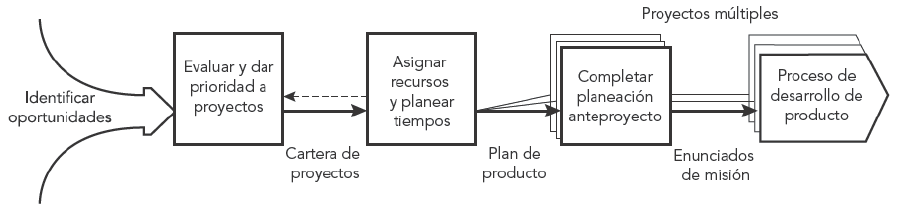
\includegraphics[width=.8\textwidth]{Figures/elproceso.png}
	\decoRule
	\caption{Proceso de planeaci\'on de un producto}
	\label{fig:elproceso}
\end{figure}

\section{Funcionalidad}
\section{Modelo de negocio}

